\lab{Least squares and Eigenvalues}{Least squares and Eigenvalues}
%TODO paragraph for the objective. Ask Mylan for a solid example.
\objective{Use least squares to fit curves to data and use QR decomposition to find eigenvalues.}
\label{lab:givens}

\section*{Least Squares}

A linear system $A\x=\b$ is \emph{overdetermined} if it has no solutions. 
In this situation, the \emph{least squares solution}, denoted as $\widehat{\x}$, is ``closest'' to a solution. 
By definition, $\widehat{\x}$ is the vector such that $A\widehat{\x}$ will equal the projection of $\b$ onto the range of $A$. 
We can compute $\widehat{\x}$ by solving the \emph{Normal Equation} $A\trp A\widehat{\x} = A\trp \b$ (see Volume 1 Section 3.8). In this lab, we will be considering matrices in $M_{m \times n}(\Bbb{R})$. Therefore, we will use the transpose instead of the Hermitian.


\subsection*{Solving the Normal Equation}
If $A$ is full rank, we can use its QR decomposition to solve the normal equation. 
In many applications, $A$ is usually full rank, including when least squares is used to fit curves to data.

Let $A=QR$ be the QR decomposition of $A$, so $R = \left(\begin{array}{c}R_0\\
0\\ \end{array} \right)$
where $R_0$ is $n \times n$, nonsingular, and upper triangular. 
It can be shown that $\widehat{\x}$ is the least squares solution to $A\x=\b$ if and only if $R_0\widehat{\x} = (Q\trp \b)[:n].$ 
Here, $(Q\trp \b)[:n]$ refers to the first $n$ rows of $Q\trp \b$.
Since $R$ is upper triangular, we can solve this equation quickly with back substitution. (see Volume 1 Exercise 3.46)

\begin{problem}
Write a function that accepts a matrix $A$ and a vector $b$ and returns the least squares solution to $Ax=b$.
Use the QR decomposition as outlined above.
Your function should use SciPy's functions for QR decomposition and for solving triangular systems, which are \li{la.qr()} and \li{la.solve_triangular()}, respectively. If you are unfamiliar with these functions, consult the documentation of these functions using object introspection.
\end{problem}

\subsection*{Using Least Squares to Fit Curves to Data}
The least squares solution can be used to find the curve of a chosen type that best fits a set of points. 

\subsubsection*{Example 1: Fitting a Line}
For example, suppose we wish to fit a general line $y=mx+b$ to the data set $\{(x_k, y_k)\}_{k=1}^n$. 
When we plug the constants $(x_k, y_k)$ into the equation $y=mx+b$, we get a system of linear equations in the unknowns $m$ and $b$. 
This system corresponds to the matrix equation
\[
\begin{pmatrix}
x_1 & 1\\
x_2 & 1\\
x_3 & 1\\
\vdots & \vdots\\
x_n & 1
\end{pmatrix}
\begin{pmatrix}
m\\
b
\end{pmatrix}=
\begin{pmatrix}
y_1\\
y_2\\
y_3\\
\vdots\\
y_n
\end{pmatrix}.
\]
Because this system has two unknowns, it is guaranteed a solution if it has two or fewer equations. 
In applications, there will usually be more than two data points, and these will probably not lie in a straight line, due to measurement error. 
Then the system will be overdetermined. 
The least squares solution to this equation will be a slope $\widehat{m}$ and $y$-intercept $\widehat{b}$ that produce a line $y = \widehat{m}x+\widehat{b}$ which best fits our data points.


%DO: spring constant as an example of this
% circle fit
% mention in this situation A will usually be full rank.
%todo: least squares and invertibiility.



%TODO: get data points that are not so close to an actual line
\begin{comment}
\begin{table}
\begin{tabular}{c|c|c|c|c|c|c|c}
displacement (cm)& 1.04  &2.03  &2.95  &3.92  &5.06  &6.00  &7.07  \\ \hline
load (dyne) & 3.11&  6.01&  9.07&  11.99 &  15.02&  17.91&  21.12\\
\end{tabular}
\end{table}
\end{comment}

Let's do an example with some actual data. 
Hooke's law from physics says that the displacement $x$ should be proportional to the load $F$, or $F = kx$ for some constant $k$.
The equation $F=kx$ describes a line with slope $k$ and $F$-intercept 0.
So the setup is similar to the setup for the general line we discussed above, except we already know $b=0$.
When we plug our seven data points $(x,F)$ into the equation $F=kx$, we get seven linear equations in $k$, corresponding to the matrix equation
\[
\begin{pmatrix}
1.04\\
2.03\\
2.95\\
3.92\\
5.06\\
6.00\\
7.07\\
\end{pmatrix}
\begin{pmatrix}k\end{pmatrix} =
\begin{pmatrix}
3.11\\
6.01\\
9.07\\
11.99\\
15.02\\
17.91\\
21.12\\
\end{pmatrix}.
\]
We expect such a linear system to be overdetermined, and in fact it is: the equation is $1.04k = 3.11$ which implies $k=2.99$, but the second equation is $2.03k = 6.01$ which implies $k=2.96$.

We can't solve this system, but its least squares solution is a ``best'' choice for $k$.
We can find the least squares solution with the SciPy function \li{linalg.lstsq()}. We pass this function the matrix $A$ and the vector $b$ from the normal equation. 
This function returns a tuple of several values, the first of which is the least squares solution, $\widehat{x}$.
\begin{lstlisting}
>>> A = np.vstack([1.04,2.03,2.95,3.92,5.06,6.00,7.07])
>>> b = np.vstack([3.11,6.01,9.07,11.99,15.02,17.91,21.12])
>>> k = la.lstsq(A, b)[0]
>>> k
array([[2.99568294]])
\end{lstlisting}
Hence, to two decimal places, $k = 3.00$.
We plot the data against the best-fit line with the following code, whose output is in Figure \ref{fig:spring_fit}

\begin{lstlisting}
>>> from matplotlib import pyplot as plt
>>> x0 = np.linspace(0,8,100)
>>> y0 = k[0]*x0
>>> plt.plot(A,b,'*',x0,y0)
>>> plt.show()
\end{lstlisting}

\begin{figure}
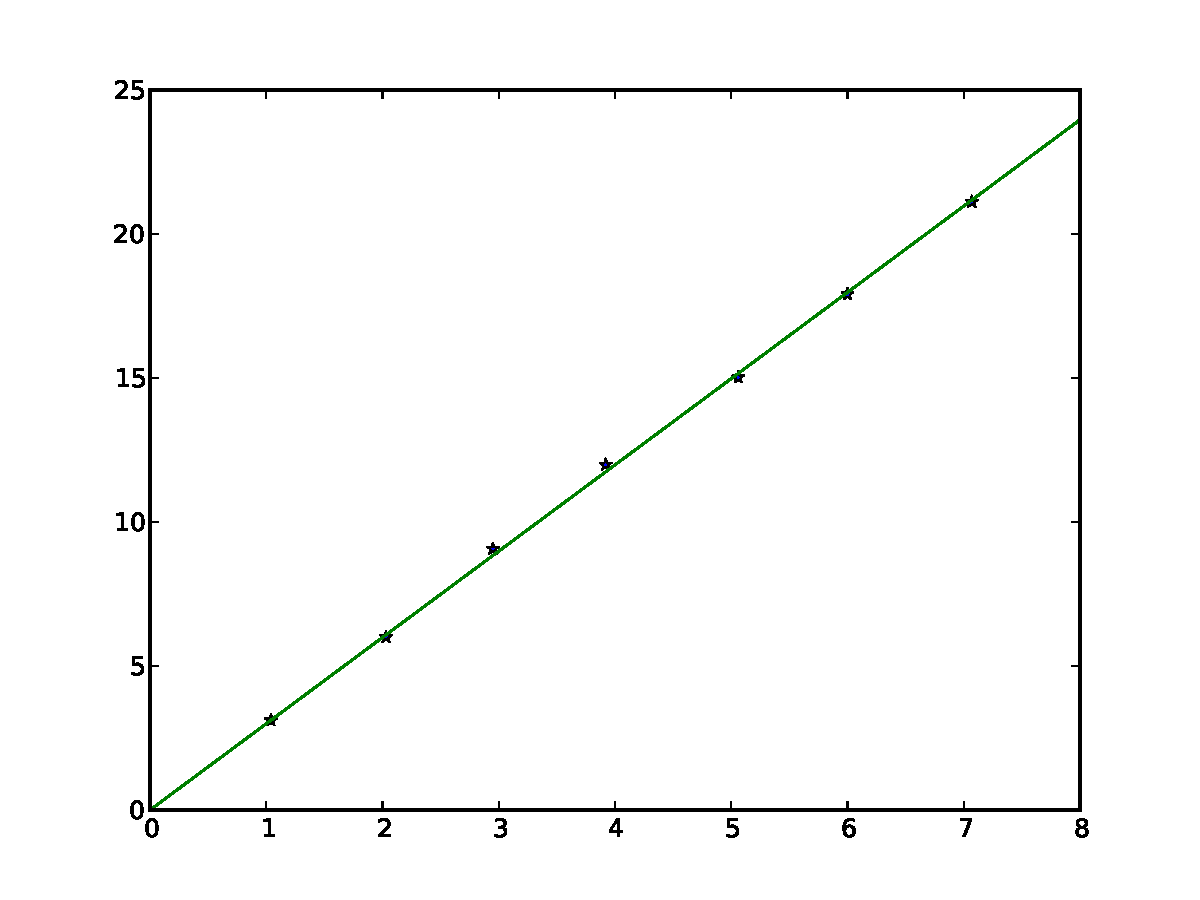
\includegraphics[width=\textwidth]{line_lstsq}
\caption{The graph of the spring data together with its linear fit.}
\label{fig:spring_fit}
\end{figure}

%TODO: find more interesting data and make a sample plot
\begin{problem}
Load the \li{linepts} array from the file \texttt{data.npz}. The following code stores this array as \li{linepts}.
\begin{lstlisting}
linepts = np.load('data.npz')['linepts']
\end{lstlisting}
The \li{linepts} array has two columns corresponding to the $x$ and $y$ coordinates of some data points.
\begin{enumerate}
\item Use least squares to fit the line $y=mx+b$ to the data.
\item Plot the data and your line on the same graph.
\end{enumerate}
\end{problem}






%
%\section*{General Line Fitting}
%
%Suppose that we wish to fit a general line, that is $y=m x+b$, to the data set
%$\{(x_k,y_k)\}^n_{k=1}$.  Assume that the line does not cross through the origin,
%as in the previous example.  Then we seek both a slope and a $y$-intercept.
%In this case, we set up the following linear system $A x = b$, or more precisely
%\[
%\begin{pmatrix}
%x_1 & 1\\
%x_2 & 1\\
%x_3 & 1\\
%\vdots & \vdots\\
%x_n & 1
%\end{pmatrix}
%\begin{pmatrix}
%m\\
%b
%\end{pmatrix}=
%\begin{pmatrix}
%y_1\\
%y_2\\
%y_3\\
%\vdots\\
%y_n
%\end{pmatrix}.
%\]
%Note that $A$ has rank $2$ as long as not all of the $x_k$ values are the same.
%Hence, the least squares solution
%is given by
%$$
%\widehat{x} = (A^HA)^{-1}A^Hb.
%$$
%In what sense does this solution give us the best fit line for the data? Recall that since $A$ is injective,
%the matrix $A(A^HA)^{-1}A^H$ is an orthogonal projector onto the range of $A$, which means that
%$A(A^HA)^{-1}A^Hb = A\widehat{x}$ is the closest vector (with respect to the 2-norm) to $b$ that lies in the
%range of $A$. That is, $\widehat{x}$ minimizes the error between $Ax$ and $b$, where the error is given
%by the distance between these vectors, $\|b-Ax\|_2$. Another way to say this is that $\widehat{x}$ gives the
%values $m$ and $b$ for which the sum of the squares of the distances from each data point $y_k$ to the value
%$y = mx_k + b$ is as small as possible.


\subsubsection*{Example 2: Fitting a Circle}
Now suppose we wish to fit a general circle to a data set $\{(x_k, y_k)\}_{k=1}^n$. Recall that the equation of a circle with radius $r$ and center $(c_1,c_2)$ is
\begin{equation}
\label{circle}
(x-c_1)^2 + (y-c_2)^2 = r^2.
\end{equation}

After expanding and rearranging this equation, we get
\begin{equation*}
\label{circle2}
2c_1x + 2c_2y + r^2 - c_1^2 - c_2^2 = x^2 + y^2.
\end{equation*}

To find $c_1$, $c_2$, and $r$ with least squares, we need \emph{linear} equations. 
The equation above is not linear because of the $r^2$, $c_1^2$, and $c_2^2$ terms. Note that it is acceptable to have the $x^2$ and $y^2$ terms because the variables in this equation are $r$, $c_1$, and $c_2$, not $x$ and $y$.
We can do a trick to make this equation linear: create a new variable $c_3$ defined by $c_3 = r^2-c_1^2-c_2^2$.

For a general data point $(x_k, y_k)$, we get the linear equation
\begin{equation*}
2c_1x_k+2c_2y_k+c_3=x_k^2+y_k^2.
\end{equation*}
Thus, we can find the best-fit circle from the least squares solution to the matrix equation

\begin{equation}\label{equ:circle_fit}
\begin{pmatrix}
2 x_1 & 2 y_1 & 1\\
2 x_2 & 2 y_2 & 1\\
\vdots & \vdots & \vdots \\
2 x_n & 2 y_n & 1
\end{pmatrix}
\begin{pmatrix}
c_1\\
c_2\\
c_3
\end{pmatrix}=
\begin{pmatrix}
x_1^2 + y_1^2\\
x_2^2 + y_2^2\\
\vdots\\
x_n^2 + y_n^2
\end{pmatrix}.
\end{equation}
If the least squares solution is $\widehat{c_1}, \widehat{c_2}$, $\widehat{c_3}$, then the best-fit circle is
\[
(x-\widehat{c_1})^2 + (y-\widehat{c_2})^2 = \widehat{c_3}+\widehat{c_1}^2+\widehat{c_2}^2.
\]

As an example, we use least squares to find the circle that best fits the nine points found in Table \ref{table:circlepts}:
\begin{table}
\begin{tabular}{c||c|c|c|c|c|c|c|c|c}
$x$& 5  &-53 & -45 &  28 & 74 & -51 &  65 & 142 & 120 \\ \hline
$y$& 11 & 35 & 139 & 170 & -7 &  87 & -24 &  64 & 131 \\
\end{tabular}
\caption{Points used in example of fitting to a circle using least squares.}
\label{table:circlepts}
\end{table}

We enter them into Python as a $9\times 2$ array.
\begin{lstlisting}
>>> P = np.array([[5,11],[-53,35],[-45,139],[28,170],[74,-7],
                [-51,87],[65,-24],[142,64],[120,131]])
\end{lstlisting}

We compute $A$ and $b$ according to Equation \ref{equ:circle_fit}.
\begin{lstlisting}
>>> A = np.hstack((2*P[:,:1], 2*P[:,1:], np.ones((9,1))))
>>> b = P[:,:1]**2 + P[:,1:]**2
\end{lstlisting}

Then we use SciPy to find the least squares solution.
\begin{lstlisting}
>>> c1, c2, c3 = la.lstsq(A, b)[0]
\end{lstlisting}

We can solve for $r$ using the relation $r^2 = c_3+c_1^2+c_2^2$.
\begin{lstlisting}
>>> r = np.sqrt(c1**2 + c2**2 + c3)
\end{lstlisting}

A good way to plot a circle is to use polar coordinates. 
Using the same variables as before, the equation for a general circle is $x=r\cos(\theta)+c_1$ and $y=r\sin(\theta)+c_2$. 
With the following code we plot the data points and our best-fit circle using polar coordinates. 
The resulting image is Figure \ref{fig:circle}.
\begin{lstlisting}
# In the polar equations for a circle, theta goes from 0 to 2*pi.
>>> theta = np.linspace(0,2*np.pi,200)
>>> plt.plot(r*np.cos(theta)+c1,r*np.sin(theta)+c2,'-',P[:,0],P[:,1],'*')
>>> plt.show()
\end{lstlisting}

\begin{figure}
\includegraphics[width=\textwidth]{newcircle.pdf}
\caption{The graph of some data and its best-fit circle.}
\label{fig:circle}
\end{figure}

\begin{comment}
\begin{problem}
Write a function \li{fitCircle} that does the following.
Load the \texttt{circlepts} array from \texttt{data.npz}.
This consists of two columns corresponding to the $x$ and $y$ values of a given
data set.  Use least squares to find the center and radius of the circle that best
fits the data.  Then plot the data points and the circle on the same graph.
The function should return nothing.
\end{problem}
\end{comment}

\begin{problem}
\leavevmode
\begin{enumerate}
\item Load the \texttt{ellipsepts} array from \texttt{data.npz}. This array has two columns corresponding to the $x$ and $y$ coordinates of some data points.
\item Use least squares to fit an ellipse to the data. 
The general equation for an ellipse is
\[
ax^2 + bx + cxy + dy + ey^2 = 1.
\]
You should get  $0.087$, $-0.141$,  $0.159$, $-0.316$, $0.366$ for $a, b, c, d,$ and $e$ respectively. Generate a plot of the resulting curve and the data points used to produce the curve.
%\item Plot the data and your line on the same graph.
\end{enumerate}

We can plot our result using polar coordinates as we did when plotting the circle. Code for visualizing your best-fit ellipse is given below. Note this bit of code plots the curve and not the data points. 

\begin{lstlisting}
    """Plots an ellipse of the form ax^2 + bx + cxy + dy + ey^2 = 1

    Input:
      X (array) - x-coordinates of all the data points.
      Y (array) - y-coordinates of all the data points.
      a,b,c,d,e (float) - the coefficients from the equation of an 
                    ellipse of the form ax^2 + bx + cxy + dy + ey^2 = 1.
    """
    def get_r(a, b, c, d, e):
        theta = np.linspace(0,2*np.pi,200)
        A = a*(np.cos(theta)**2) + c*np.cos(theta)*np.sin(theta) + e*(np.sin(theta)**2)
        B = b*np.cos(theta) + d*np.sin(theta)
        r = (-B + np.sqrt(B**2 + 4*A))/(2*A)
        return r, theta
        
    r,theta = get_r(a,b,c,d,e)
    plt.plot(r*np.cos(theta), r*np.sin(theta), color = "r")
    plt.plot(X,Y,".", color = "b")
    plt.axes().set_aspect('equal', 'datalim')
    plt.show()
\end{lstlisting}

\end{problem}

%TODO: keep this?
\begin{comment}
In these Least Squares problems, we have found best fit lines and ellipses relative to the 2-norm.
It is possible to generalize the idea of best fit curves relative to other norms.
See Figure \ref{Fig:ellipse} for an illustration of this.

\begin{figure}[h]
\label{ellipsefit}
\centering
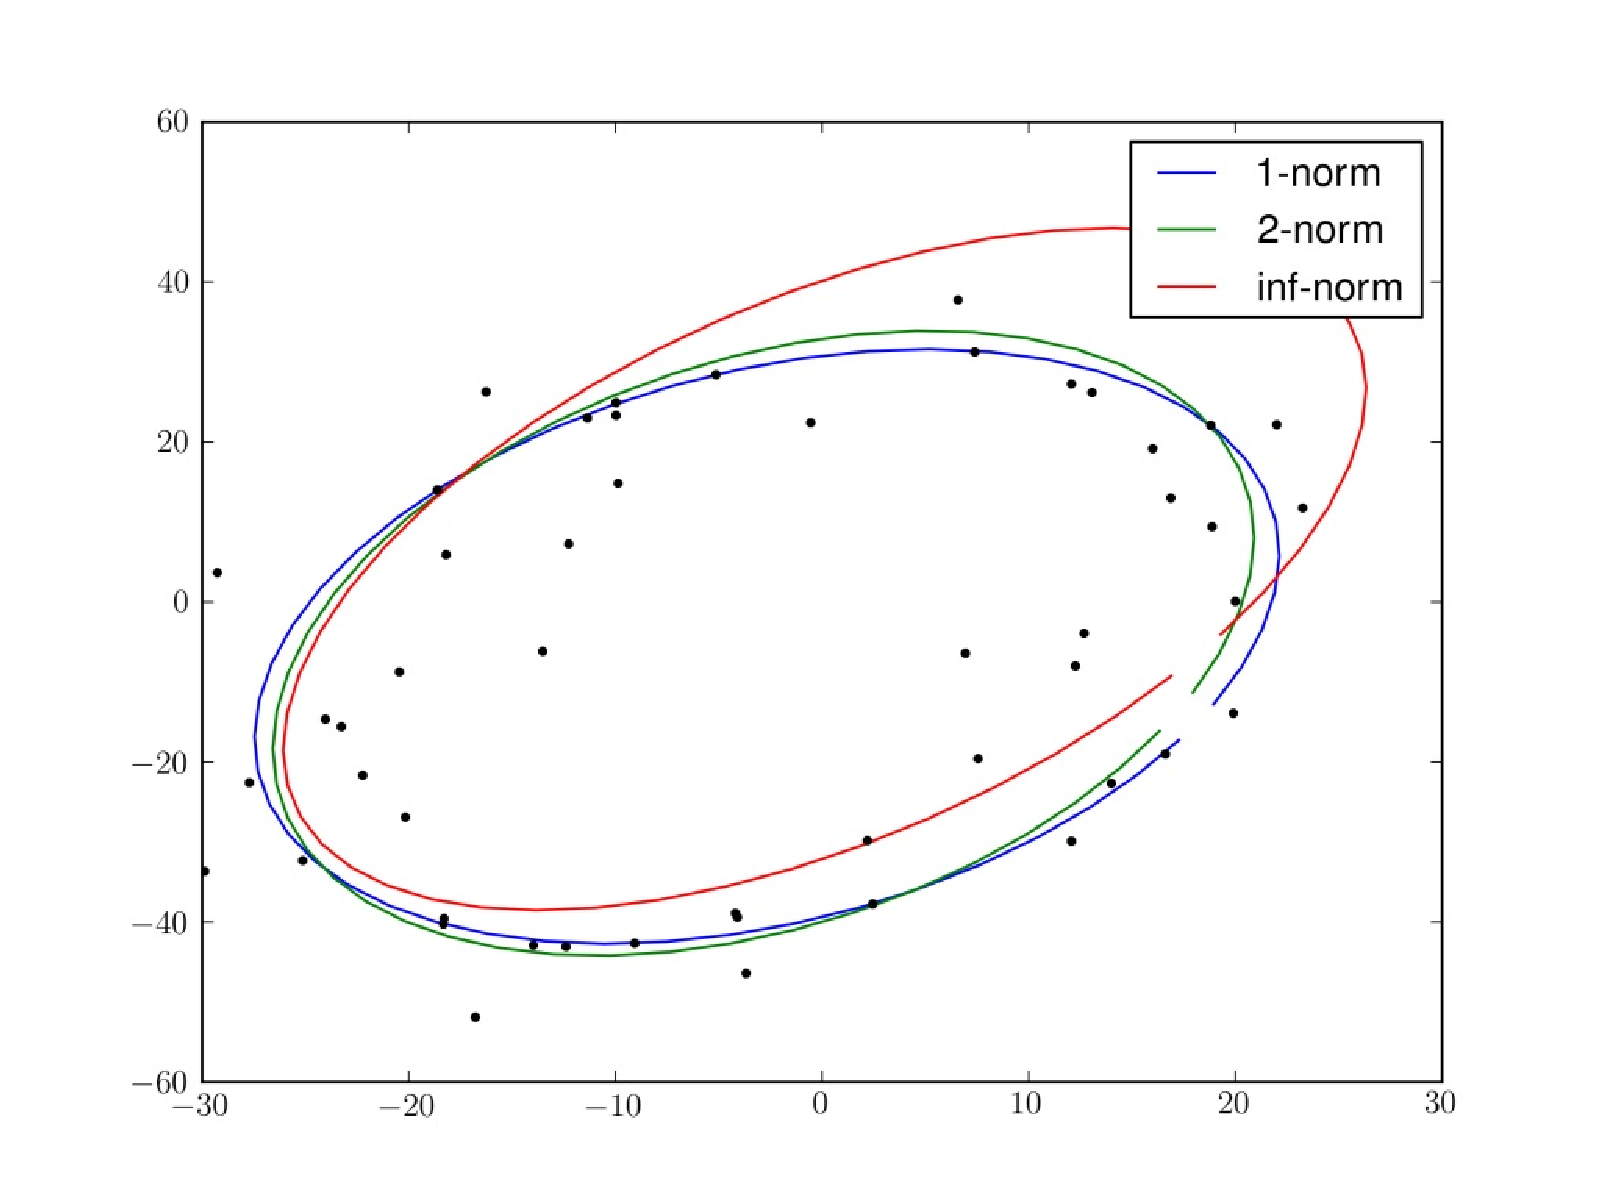
\includegraphics[width=\textwidth]{ellipsefit.pdf}
\caption{Fitting an ellipse using different norms.}
\label{Fig:ellipse}
\end{figure} 
\end{comment}

\begin{comment}
\section*{Loading Data from .npz Files}
For Least Squares problems as well as in many other contexts, loading data is often a necessary step before
proceeding with further analysis. Here we briefly review another data format in Python and the commands used
to load the data.

A \li{.npz} file is a compressed binary file that contains an archive of NumPy data structures.
A given file may therefore contain several arrays, each array associated with a unique string that identifies it.
When you load a \li{.npz} file in Python, a dictionary-like object is returned, and you can access the data by
providing the appropriate key. Note that when you load a \li{.npz} file, you must also be sure to close it when
you are finished. This is taken care of automatically if you use the \li{with ... as} keywords.

As an example, suppose that we have a file named \li{grades.npz} that contains several arrays, each giving the
homework scores of a particular student in a particular class. Assuming that one of the arrays is associated with
the key \li{'Abe'}, we can load this array in the following way:

\begin{lstlisting}
>>> with np.load('grades.npz') as grades:
>>>     abe_grades = grades['Abe']
>>> abe_grades
array([ 10.,  10.,  10.,  10.,  10.,  10.,  10.,  10.,  10.,  10.])
\end{lstlisting}

You will need to apply this technique in the next problem.

\end{comment}

\section*{Computing Eigenvalues}
The eigenvalues of a matrix are the roots of its characteristic polynomial. 
Thus, to find the eigenvalues of an $n \times n$ matrix, we must compute the roots of a degree-$n$ polynomial. 
This is easy for small $n$. 
For example, if $n=2$ the quadratic equation can be used to find the eigenvalues. 
However, Abel's Impossibility Theorem says that no such formula exists for the roots of a polynomial of degree 5 or higher.

\begin{theorem}[Abel's Impossibility Theorem]
There is no general algebraic solution for solving a polynomial equation of degree $n\geq5$.
\label{thm:Abel}
\end{theorem}

Thus, it is impossible to write an algorithm that will exactly find the eigenvalues of an arbitrary matrix. 
(If we could write such an algorithm, we could also use it to find the roots of polynomials, contradicting Abel's theorem.) 
This is a significant result. 
It means that we must find eigenvalues with \emph{iterative methods}, methods that generate sequences of approximate values converging to the true value.

\subsection*{The Power Method}
There are many iterative methods for finding eigenvalues. 
The power method finds an eigenvector corresponding to the \emph{dominant} eigenvalue of a matrix, if such an eigenvalue exists.
The dominant eigenvalue of a matrix is the unique eigenvalue of greatest magnitude.

To use the power method on a matrix $A$, begin by choosing a vector $\x_0$ such that $\|\x_0\|=1$. Then recursively define
\[
x_{k+1}=\frac{Ax_k}{\norm{Ax_k}}.
\]
If 
\begin{itemize}
\item $A$ has a dominant eigenvalue $\lambda$, and
\item the projection of $\x_0$ into the subspace spanned by the eigenvectors corresponding to $\lambda$ is nonzero,
\end{itemize}
then the vectors $\x_0, \x_1, \x_2, \ldots$ will converge to an eigenvector of $A$ corresponding to $\lambda$. 
(See [TODO: ref textbook] for a proof when $A$ is semisimple, or [TODO: ref something else] for a proof in the general case.)

If all entries of $A$ are positive, then $A$ will always have a dominant eigenvalue (see [TODO: ref something!] for a proof). 
There is no way to guarantee that the second condition is met, but if we choose $\x_0$ randomly, it will almost always satisfy this condition.

Once you know that $\x$ is an eigenvector of $A$, the corresponding eigenvalue is equal to the \emph{Rayleigh quotient}
\[
\lambda = \frac{\langle Ax, x \rangle}{\|\x\|^2}.
\]



\begin{problem}
Write a function that implements the power method to compute an eigenvector. Your function should
\begin{enumerate}
\item Accept a matrix and a tolerance \li{tol}.
\item Start with a random vector.
\item Use the 2-norm wherever a norm is needed (use \li{la.norm()}).
\item Repeat the power method until the vector changes by less than the tolerance. In mathematical notation, you are defining $x_0, x_1, \ldots x_k$, and your function should stop when $\|x_{k+1}-x_k\| < \text{tol}$.
\item Return the found eigenvector and the corresponding eigenvalue (use \li{np.inner()}).
\end{enumerate} 
Test your function on positive matrices.
\end{problem}

\begin{comment}
An overview of the proof of the method is that you can write a matrix in Jordan Conical form $A=VJV^{-1}$ where $V$ is the matrix of the generalized eigenspaces. 
But the first column is is the eigenvector corresponding to largest eigenvalue and $J$ is a upper trianglar matrix of eigenvalues and ones.
Note that $A^k=VJ^kV^{-1}$. The limit as $k \rightarrow \infty$ of $(\frac{1}{\lambda_1}J)^k$ is a matrix of all zeros except for a one in the upper right hand corner. 
So $(\frac{A}{\norm{A}})^k \approx VJ^kV^{-1}$ So the largest eigenvalue dominates.
\end{comment}

\subsection*{The QR Algorithm}
The disadvantage of the power method is that it only finds the largest eigenvector and a corresponding eigenvalue. 
To use the QR algorithm, let $A_0=A$. Then let $Q_kR_k$ be the QR decomposition of $A_k$, and recursively define 
\[
A_{k+1}=R_kQ_k.
\] 
Then $A_0, A_1, A_2, \ldots $ will converge to a matrix of the form
\begin{equation*}
\label{eq:Schur form}
S =
     \begin{pmatrix}
          S_1 &* & \cdots & * \\
           0     &S_2  &  \ddots & \vdots \\
           \vdots  & \ddots & \ddots & *  \\
           0 & \cdots & 0 & S_m
    \end{pmatrix}
\end{equation*}
where $S_i$ is a $1\times1$ or $2\times2$ matrix.\footnote{If $S$ is upper triangular (i.e., all $S_i$ are $1\times1$ matrices), then $S$ is the \emph{Schur form} of $A$. 
If some $S_i$ are $2\times2$ matrices, then $S$ is the \emph{real Schur form} of $A$.} 
The eigenvalues of $A$ are the eigenvalues of the $S_i$.

This algorithm works for three reasons. First, 
\[
Q_k^{-1}A_kQ_k = Q_k^{-1}(Q_kR_k)Q_k = (Q_k^{-1}Q_k)(R_kQ_k) = A_{k+1},
\]
so $A_k$ is similar to $A_{k+1}$. 
Because similar matrices have the same eigenvalues, $A_k$ has the same eigenvalues as $A$. 
Second, each iteration of the algorithm transfers some of the ``mass'' from the lower to the upper triangle. 
This is what makes $A_0, A_1, A_2, \ldots$ converge to a matrix $S$ which has the described form. 
Finally, since $S$ is block upper triangular, its eigenvalues are just the eigenvalues of its diagonal blocks (the $S_i$).

A $2 \times 2$ block will occur in $S$ when $A$ is real but has complex eigenvalues. 
In this case, the complex eigenvalues occur in conjugate pairs, each pair corresponding to a $2 \times 2$ block on the diagonal of $S$.


\subsubsection*{Hessenberg Preconditioning}
Often, we ``precondition'' a matrix by putting it in upper Hessenberg form before passing it to the QR algorithm. 
This is always possible because every matrix is similar to an upper Hessenberg matrix (see Lab \ref{}). 
Hessenberg preconditioning is done for two reasons.

First, the QR algorithm converges much faster on upper Hessenberg matrices because they are already close to triangular matrices. 

Second, an iteration of the QR algorithm can be computed in $\mathcal{O}(n^2)$ time on an upper Hessenberg matrix, as opposed to $\mathcal{O}(n^3)$ time on a regular matrix. 
This is because so many entries of an upper Hessenberg matrix are 0.
If we apply the QR algorithm to an upper Hessenberg matrix $H$, then this speed-up happens in each iteration of the algorithm, since if $H = QR$ is the QR decomposition of $H$ then $RQ$ is also upper Hessenberg.


\begin{problem}
Write a function that implements the QR algorithm with Hessenberg preconditioning as described above. 
Do this as follows.
\begin{enumerate}
\item Accept a matrix \li{A}, a number of iterations \li{niter}, and a tolerance \li{tol}.
\item Put \li{A} in Hessenberg form using \li{la.hessenberg()}.
\item Compute the matrix $S$ by performing the QR algorithm \li{niter} times. 
Use the function \li{la.qr()} to compute the QR decomposition.
\item Iterate through the diagonal of $S$ from top to bottom to compute its eigenvalues. 
For each diagonal entry,
\begin{enumerate}
\item If this is the last diagonal entry, then it is an eigenvalue.
\item If the entry below this one has absolute value less than \li{tol}, assume this is a $1\times 1$ block. 
Then the current entry is an eigenvalue.
\item Otherwise, the current entry is at the top left corner of a $2 \times 2$ block. 
Calculate the eigenvalues of this block. 
Use the \li{sqrt} function from the scimath library to find the square root of a negative number. 
You can import this library with the line \li{from numpy.lib import scimath}.
\end{enumerate}
\item Return the (approximate) eigenvalues of \li{A}.
\end{enumerate}
You can check your function on the matrix
\[
\begin{pmatrix}
 4 &  12 & 17 &  -2 \\
-5.5& -30.5 & -45.5 &  9.5\\
 3. &  20. & 30. &  -6. \\
1.5 &  1.5&   1.5&   1.5
       \end{pmatrix},
\]
which has eigenvalues $1+2i, 1-2i, 3$, and 0. You can also check your function on random matrices against \li{la.eig()}.
\label{prob:qr_solver}
\end{problem}


\begin{comment}
\begin{problem}
\label{prob:QR_eig_hessenberg}
Write a version of the QR algorithm that performs the QR algorithm by computing the Hessenberg form of a matrix, then computing various QR decompositions of the Hessenberg form of the matrix.
Use your solutions to \ref{prob:hessenberg} (where you computed the Hessenberg form of a matrix) and Problem \ref{prob:givens_hessenberg_modified} to do the necessary computations (where you computed the QR decomposition of a Hessenberg matrix and wrote code for multiplication by $Q$ that works in $\mathcal{O} \left( n^2 \right)$ time).
The solution to Problem \ref{prob:givens_hessenberg_modified} is especially important because it allows the compution of each QR decomposition and each $R Q = \left( Q^T R^T \right)$ in $\mathcal{O} \left( n^2 \right)$ time.
\end{problem}
\end{comment}

\begin{comment}
\begin{problem}
If $A$ is normal, its Schur form is diagonal.
For normal $A$, have your function additionally output the eigenvector corresponding to each eigenvalue.
Hint 1: Test your function on Hermitian and real symmetric matrices; they are both normal.
Hint 2: Your work in Problem \ref{problem:similarity proof} will help.
You have already made all the necessary calculations, you just need to store the information correctly.
\end{problem}
\end{comment}

\begin{comment}
\begin{problem}
Test your implementation with random matrices.
Try real-valued and symmetric matrices.
Compare your output to the output from the eigenvalue solver.
How many iterations are necessary?
How large can $A$ be?
\end{problem}
\end{comment}

The QR algorithm as described in this lab is not often used. 
Instead, modern computer packages use the implicit QR algorithm, which is an improved version of the QR algorithm.

Lastly, iterative methods besides the power method and QR method are often used to find eigenvalues.
Arnoldi iteration is similar to the QR algorithm but exploits sparsity.
Other methods include the Jacobi method and the Rayleigh quotient method.
